\chapter{Abordagem}

Neste cap\'itulo ser\'a realizada uma minuciosa an\'alise ao jogo Hamle e ao m\'etodo de resolu\c{c}\~ao implementado. \\
Come\c{c}aremos por descrever as vari\'aveis de decis\~ao e seus respetivos dom\'inios, seguidas de uma avalia\c{c}\~ao das restri\c{c}\~oes a serem trabalhadas. Ser\'a ainda indicada a forma de avalia\c{c}\~ao da solu\c{c}\~ao obtida bem como a estrat\'egia de pesquisa aplicada ao $labeling$, no c\'alculo das poss\'iveis solu\c{c}\~oes.

\section{Vari\'aveis de Decis\~ao}

Como variavel de decis\~ao, \'e gerada, na fun\c{c}\~ao $solution$, uma lista denominada $Result$ a qual ter\'a a dimens\~ao de um tabuleiro, simulando a jun\c{c}\~ao de uma linha do tabuleiro ao final da anterior, isto \'e, tendo como exemplo um tabuleiro NxN, temos que $length(Result, Length)$, onde $Length = N*N$.\\
O dom\'inio da vari\'avel $Result$ ser\'a compreendido entre 0 e $N-1$, sendo que 0 representar\'a as c\'elulas vazias e os algarismos compreendidos entre 1 e $N-1$ corresponder\~ao \`a desloca\c{c}\~ao respetiva a cada pe\c{c}a preta presente no tabuleiro original. Sendo assim, a cada algarismo $V$ presente num dado \'indice $I$ da lista $Result$, ent\~ao, necess\'ariamente, existir\'a na lista original (representativa do estado inicial do tabuleiro), o mesmo valor $N$ no \'indice $I + N*V$ (deslocamento para baixo), no \'indice $I - N*V$ (deslocamento para cima), no \'indice $I + V$ (deslocamento para a direita) ou no \'indice $I - V$ (deslocamento para a esquerda). N\~ao pode deixar de ser referido que no deslocamento horizontal, o \'indice de destino dever\'a corresponder \`a mesma linha do \'indice de origem, pelo que $floor(I\small{destino} / N) = floor(I\small{origem} / N)$.\\ \\ \\ \\ \\ \\ \\ 

\section{Restri\c{c}\~oes}

No presente subcap\'itulo, descreveremos a implementa\c{c}\~ao das diversas restri\c{c}\~oes que constituem o problema da determina\c{c}\~ao de solu\c{c}\~oes para o jogo Hamle. Para qualquer umas das restri\c{c}\~oes foi criada uma fun\c{c}\~ao auxiliar para o respetivo c\'alculo ou verifica\c{c}\~ao.

\subsection{Pe\c{c}as n\~ao-adjacentes}
Esta \'e a restri\c{c}\~ao mais simples das que consistem o jogo. 
\\ \\
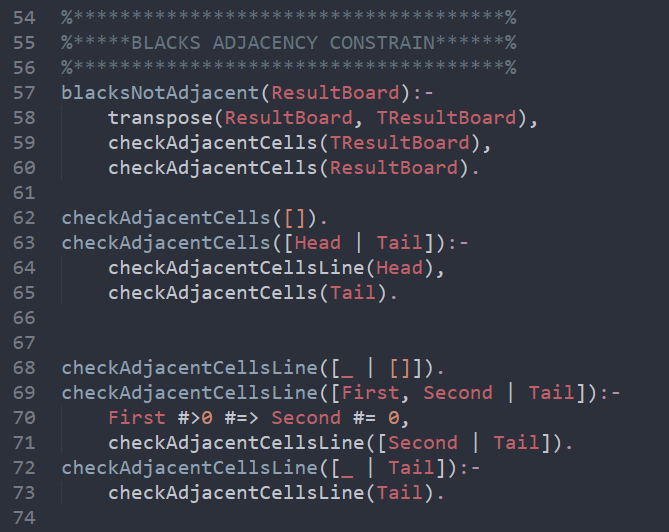
\includegraphics[scale=0.5]{no-adjacents.png}
\\ \\
Tendo como argumento $ResultBoard$ (uma lista de listas respetiva \`a divis\~ao da lista de vari\'aveis $Result$, sendo que cada sublista representa uma linha do tabuleiro), temos como objetivo garantir que nenhuma posi\c{c}\~ao com valor superior a 0 tenha na sua proximidade outro valor igualmente superior a 0. Desse modo, ao percorrer uma linha do tabuleiro (sublista de $ResultBoard$), impomos que, dada uma posi\c{c}\~ao, referente a uma pe\c{c}a preta, dever\'a ser seguida de um espa\c{c}o em branco (valor 0). Uma vez que esta condi\c{c}\~ao se verifica tanto na horizontal como na vertical, gera-se uma matriz transposta a $ResultBoard$ que posteriormente ser\'a verificada com as restri\c{c}\~ao em an\'alise.
\\ \\ \\ \\ \\ \\ \\ \\

\subsection{Movimento de pe\c{c}as pretas}
Relativamente ao movimento das pe\c{c}as pretas, podemos dividir a restri\c{c}\~ao em duas fases: a verifica\c{c}\~ao das possibilidades de desloca\c{c}\~ao de cada pe\c{c}a e a respetiva valida\c{c}\~ao e coloca\c{c}\~ao em tabuleiro.
\\ \\
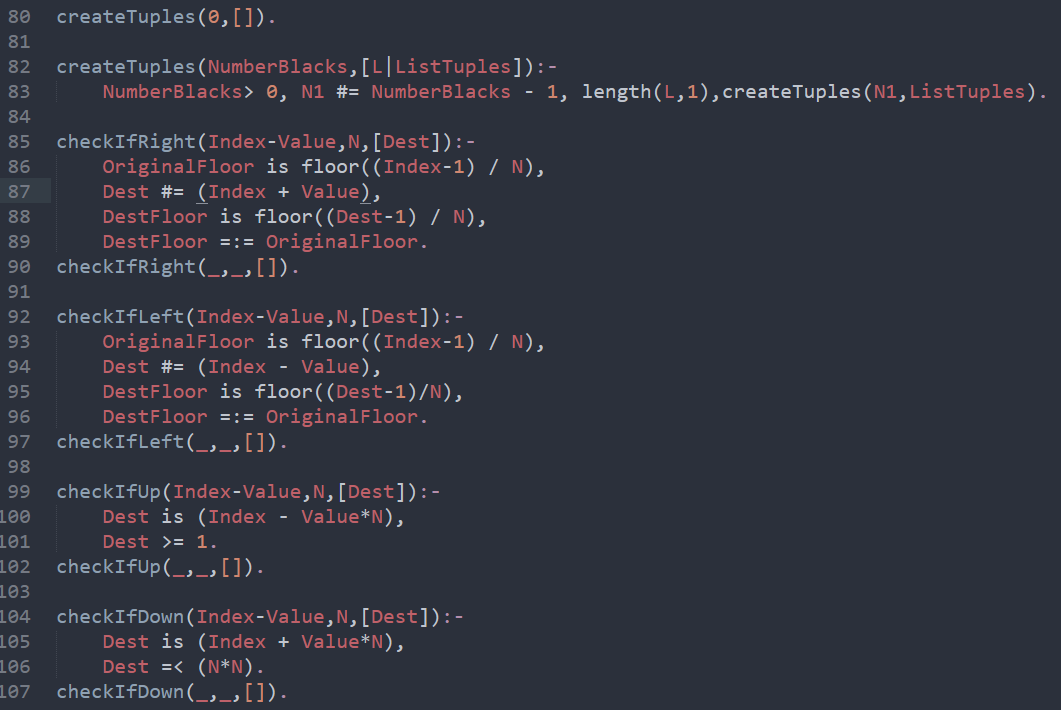
\includegraphics[scale=0.5]{movement-checkers.png}
\\ 
Nestas fun\c{c}\~oes s\~ao recriadas as possiveis posi\c{c}\~oes que cada pe\c{c}a poder\'a ocupar, dependendo da c\'elula onde se encontra e da dire\c{c}\~ao na qual se poder\'a deslocar. Estas posi\c{c}\~oes a serem determinadas s\~ao calculadas com base no \'indice de cada c\'elula, pelo que se recorre \`a fun\c{c}\~ao $floor/1$ para considerar que, em caso de deslocamento horizontal, o indice de origem corresponde \`a mesma linha de tabuleiro que o \'indice de destino.
\\ \\
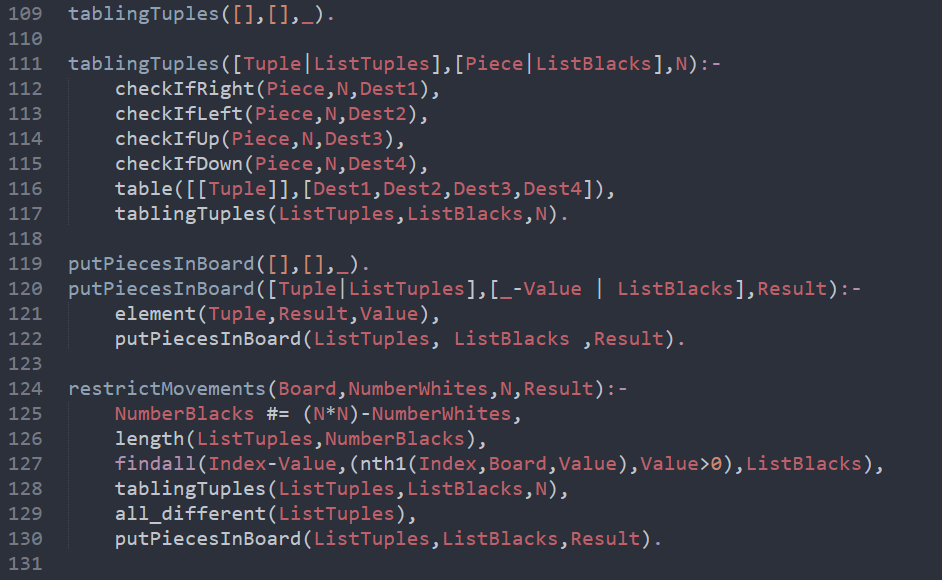
\includegraphics[scale=0.4]{movement-validators.png}
\\ \\
Ap\'os a determina\c{c}\~ao dos poss\'iveis destinos para cada pe\c{c}a preta, procede-se \`a coloca\c{c}\~ao de cada uma no seu novo local recorrendo ao $table$, que nos permite criar um subdom\'inio relativo a cada objeto, com as diferentes posi\c{c}\~oes para onde se poder\'a mover. Neste momento, \'e tamb\'em restringida a possibilidade de quaisquer pe\c{c}as ocuparem a mesma c\'elula.

\subsection{Interconectividade das c\'elulas vazias}
Embora o conceito de interconectividade n\~ao seja complicado de assimilar, n\~ao fomos capazes de implementar corretamente a restri\c{c}\~ao pretendida neste ponto.
Na imagem seguinte apresentamos o algoritmo que nos permite detetar o n\'umero de c\'elulas vazias \`as quais podemos aceder, partindo de uma posi\c{c}\~ao livre.
\\ \\ 
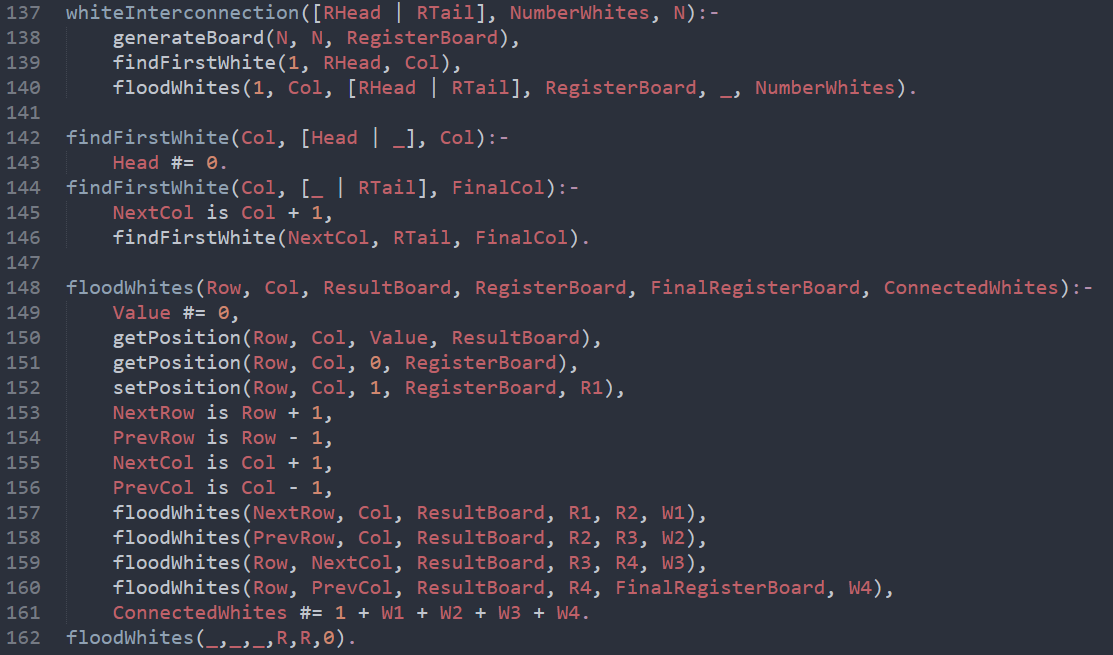
\includegraphics[scale= 0.5]{white-interconnection.png}
\\ \\ \\ \\ \\
O objetivo do nosso grupo seria, ap\'os detetar a primeira c\'elula vazia da primeira linha de tabuleiro, expandir a procura atrav\'es das c\'elulas desocupadas na vizinhan\c{c}a dessa primeira posi\c{c}\~ao, recorrendo ao aux\'ilio de um tabuleiro de registo, que nos identificaria as c\'elulas anteriormente visitadas durante o processo.\\
Tendo testado o algoritmo, podemos assegurar que se encontra funcional, embora n\~ao seja vi\'avel ao pretendido neste projeto.

\section{Fun\c{c}\~ao de Avalia\c{c}\~ao}
Ap\'os a execu\c{c}\~ao das restri\c{c}\~oes e alcance de uma solu\c{c}\~ao que as satisfa\c{c}a, ser\'a poss\'ivel visualizar um novo tabuleiro com a respetiva movimenta\c{c}\~ao de cada pe\c{c}a preta. Tal poder\'a ser observado uma vez que cada pe\c{c}a conservar\'a o seu valor de deslocamento, assim como no tabuleiro original.

\section{Estrat\'egia de Pesquisa}
Foi utilizada, como estrat\'egia de etiquetagem, o modo $default$ da fun\c{c}\~ao $labeling$, ou seja, recorre-se \`as op\c{c}\~oes $leftmost$, $step$, $up$ e $all$.

